\documentclass[twoside]{book}

% Packages required by doxygen
\usepackage{calc}
\usepackage{doxygen}
\usepackage{graphicx}
\usepackage[utf8]{inputenc}
\usepackage{makeidx}
\usepackage{multicol}
\usepackage{multirow}
\usepackage{textcomp}
\usepackage[table]{xcolor}

% Font selection
\usepackage[T1]{fontenc}
\usepackage{mathptmx}
\usepackage[scaled=.90]{helvet}
\usepackage{courier}
\usepackage{amssymb}
\usepackage{sectsty}
\renewcommand{\familydefault}{\sfdefault}
\allsectionsfont{%
  \fontseries{bc}\selectfont%
  \color{darkgray}%
}
\renewcommand{\DoxyLabelFont}{%
  \fontseries{bc}\selectfont%
  \color{darkgray}%
}

% Page & text layout
\usepackage{geometry}
\geometry{%
  a4paper,%
  top=2.5cm,%
  bottom=2.5cm,%
  left=2.5cm,%
  right=2.5cm%
}
\tolerance=750
\hfuzz=15pt
\hbadness=750
\setlength{\emergencystretch}{15pt}
\setlength{\parindent}{0cm}
\setlength{\parskip}{0.2cm}
\makeatletter
\renewcommand{\paragraph}{%
  \@startsection{paragraph}{4}{0ex}{-1.0ex}{1.0ex}{%
    \normalfont\normalsize\bfseries\SS@parafont%
  }%
}
\renewcommand{\subparagraph}{%
  \@startsection{subparagraph}{5}{0ex}{-1.0ex}{1.0ex}{%
    \normalfont\normalsize\bfseries\SS@subparafont%
  }%
}
\makeatother

% Headers & footers
\usepackage{fancyhdr}
\pagestyle{fancyplain}
\fancyhead[LE]{\fancyplain{}{\bfseries\thepage}}
\fancyhead[CE]{\fancyplain{}{}}
\fancyhead[RE]{\fancyplain{}{\bfseries\leftmark}}
\fancyhead[LO]{\fancyplain{}{\bfseries\rightmark}}
\fancyhead[CO]{\fancyplain{}{}}
\fancyhead[RO]{\fancyplain{}{\bfseries\thepage}}
\fancyfoot[LE]{\fancyplain{}{}}
\fancyfoot[CE]{\fancyplain{}{}}
\fancyfoot[RE]{\fancyplain{}{\bfseries\scriptsize Generated on Tue May 5 2015 16\-:50\-:28 for D\-S\-Epp by Doxygen }}
\fancyfoot[LO]{\fancyplain{}{\bfseries\scriptsize Generated on Tue May 5 2015 16\-:50\-:28 for D\-S\-Epp by Doxygen }}
\fancyfoot[CO]{\fancyplain{}{}}
\fancyfoot[RO]{\fancyplain{}{}}
\renewcommand{\footrulewidth}{0.4pt}
\renewcommand{\chaptermark}[1]{%
  \markboth{#1}{}%
}
\renewcommand{\sectionmark}[1]{%
  \markright{\thesection\ #1}%
}

% Indices & bibliography
\usepackage{natbib}
\usepackage[titles]{tocloft}
\setcounter{tocdepth}{3}
\setcounter{secnumdepth}{5}
\makeindex

% Hyperlinks (required, but should be loaded last)
\usepackage{ifpdf}
\ifpdf
  \usepackage[pdftex,pagebackref=true]{hyperref}
\else
  \usepackage[ps2pdf,pagebackref=true]{hyperref}
\fi
\hypersetup{%
  colorlinks=true,%
  linkcolor=blue,%
  citecolor=blue,%
  unicode%
}

% Custom commands
\newcommand{\clearemptydoublepage}{%
  \newpage{\pagestyle{empty}\cleardoublepage}%
}


%===== C O N T E N T S =====

\begin{document}

% Titlepage & ToC
\hypersetup{pageanchor=false}
\pagenumbering{roman}
\begin{titlepage}
\vspace*{7cm}
\begin{center}%
{\Large D\-S\-Epp }\\
\vspace*{1cm}
{\large Generated by Doxygen 1.8.6}\\
\vspace*{0.5cm}
{\small Tue May 5 2015 16:50:28}\\
\end{center}
\end{titlepage}
\clearemptydoublepage
\tableofcontents
\clearemptydoublepage
\pagenumbering{arabic}
\hypersetup{pageanchor=true}

%--- Begin generated contents ---
\chapter{The D\-S\-Epp library documentation}
\label{index}\hypertarget{index}{}\input{index}
\chapter{Namespace Index}
\input{namespaces}
\chapter{Hierarchical Index}
\section{Class Hierarchy}
This inheritance list is sorted roughly, but not completely, alphabetically\-:\begin{DoxyCompactList}
\item \contentsline{section}{C\-\_\-\-Abs\-Diagram}{\pageref{class_c___abs_diagram}}{}
\begin{DoxyCompactList}
\item \contentsline{section}{B\-S\-E\-:\-:C\-\_\-\-B\-S\-E}{\pageref{class_b_s_e_1_1_c___b_s_e}}{}
\begin{DoxyCompactList}
\item \contentsline{section}{B\-S\-E\-:\-:C\-\_\-\-B\-S\-E\-\_\-\-Two\-Body}{\pageref{class_b_s_e_1_1_c___b_s_e___two_body}}{}
\begin{DoxyCompactList}
\item \contentsline{section}{B\-S\-E\-:\-:C\-\_\-\-B\-S\-E\-\_\-\-Matrix}{\pageref{class_b_s_e_1_1_c___b_s_e___matrix}}{}
\begin{DoxyCompactList}
\item \contentsline{section}{B\-S\-E\-:\-:C\-\_\-\-B\-S\-E\-\_\-\-Pseudo\-Scalar}{\pageref{class_b_s_e_1_1_c___b_s_e___pseudo_scalar}}{}
\item \contentsline{section}{B\-S\-E\-:\-:C\-\_\-\-B\-S\-E\-\_\-\-Scalar}{\pageref{class_b_s_e_1_1_c___b_s_e___scalar}}{}
\item \contentsline{section}{B\-S\-E\-:\-:C\-\_\-\-B\-S\-E\-\_\-\-Vector}{\pageref{class_b_s_e_1_1_c___b_s_e___vector}}{}
\end{DoxyCompactList}
\end{DoxyCompactList}
\end{DoxyCompactList}
\item \contentsline{section}{Kernels\-:\-:C\-\_\-\-Abstract\-Kernel}{\pageref{class_kernels_1_1_c___abstract_kernel}}{}
\begin{DoxyCompactList}
\item \contentsline{section}{Kernels\-:\-:C\-\_\-\-Two\-Quark\-Kernel}{\pageref{class_kernels_1_1_c___two_quark_kernel}}{}
\begin{DoxyCompactList}
\item \contentsline{section}{Kernels\-:\-:C\-\_\-\-Kernel\-\_\-\-R\-L}{\pageref{class_kernels_1_1_c___kernel___r_l}}{}
\item \contentsline{section}{Kernels\-:\-:C\-\_\-\-Kernel\-\_\-\-R\-L\-\_\-\-P\-S}{\pageref{class_kernels_1_1_c___kernel___r_l___p_s}}{}
\end{DoxyCompactList}
\end{DoxyCompactList}
\item \contentsline{section}{Propagators\-:\-:C\-\_\-\-Propagator}{\pageref{class_propagators_1_1_c___propagator}}{}
\begin{DoxyCompactList}
\item \contentsline{section}{Propagators\-:\-:C\-\_\-\-Gluon}{\pageref{class_propagators_1_1_c___gluon}}{}
\item \contentsline{section}{Propagators\-:\-:C\-\_\-\-Quark}{\pageref{class_propagators_1_1_c___quark}}{}
\begin{DoxyCompactList}
\item \contentsline{section}{Propagators\-:\-:C\-\_\-\-Bottom\-\_\-\-Quark}{\pageref{class_propagators_1_1_c___bottom___quark}}{}
\item \contentsline{section}{Propagators\-:\-:C\-\_\-\-Charm\-\_\-\-Quark}{\pageref{class_propagators_1_1_c___charm___quark}}{}
\item \contentsline{section}{Propagators\-:\-:C\-\_\-\-Down\-\_\-\-Quark}{\pageref{class_propagators_1_1_c___down___quark}}{}
\item \contentsline{section}{Propagators\-:\-:C\-\_\-\-Strange\-\_\-\-Quark}{\pageref{class_propagators_1_1_c___strange___quark}}{}
\item \contentsline{section}{Propagators\-:\-:C\-\_\-\-Test\-\_\-\-Quark}{\pageref{class_propagators_1_1_c___test___quark}}{}
\item \contentsline{section}{Propagators\-:\-:C\-\_\-\-Up\-\_\-\-Quark}{\pageref{class_propagators_1_1_c___up___quark}}{}
\end{DoxyCompactList}
\end{DoxyCompactList}
\end{DoxyCompactList}
\item \contentsline{section}{C\-\_\-\-Abstract\-Builder}{\pageref{class_c___abstract_builder}}{}
\begin{DoxyCompactList}
\item \contentsline{section}{C\-\_\-\-Meson\-Builder}{\pageref{class_c___meson_builder}}{}
\end{DoxyCompactList}
\item \contentsline{section}{Interpolation\-:\-:C\-\_\-\-Base\-\_\-interp}{\pageref{class_interpolation_1_1_c___base__interp}}{}
\begin{DoxyCompactList}
\item \contentsline{section}{Interpolation\-:\-:C\-\_\-\-Bary\-Rat\-\_\-interp}{\pageref{class_interpolation_1_1_c___bary_rat__interp}}{}
\end{DoxyCompactList}
\item \contentsline{section}{C\-\_\-\-Binder}{\pageref{class_c___binder}}{}
\item \contentsline{section}{B\-S\-E\-:\-:C\-\_\-\-Bound\-State\-\_\-parameters}{\pageref{class_b_s_e_1_1_c___bound_state__parameters}}{}
\item \contentsline{section}{B\-S\-E\-:\-:C\-\_\-\-B\-S\-E\-\_\-\-Factory}{\pageref{class_b_s_e_1_1_c___b_s_e___factory}}{}
\item \contentsline{section}{C\-\_\-\-Dedic\-Mem\-\_\-\-Abs}{\pageref{class_c___dedic_mem___abs}}{}
\begin{DoxyCompactList}
\item \contentsline{section}{C\-\_\-\-Dedic\-Mem\-\_\-\-B\-S\-E}{\pageref{class_c___dedic_mem___b_s_e}}{}
\item \contentsline{section}{C\-\_\-\-Dedic\-Mem\-\_\-\-Kernel}{\pageref{class_c___dedic_mem___kernel}}{}
\item \contentsline{section}{C\-\_\-\-Dedic\-Mem\-\_\-\-Quark}{\pageref{class_c___dedic_mem___quark}}{}
\end{DoxyCompactList}
\item \contentsline{section}{Propagators\-:\-:C\-\_\-\-Gluon\-\_\-\-Factory}{\pageref{class_propagators_1_1_c___gluon___factory}}{}
\item \contentsline{section}{C\-\_\-\-Gradiend\-\_\-\-Descent}{\pageref{class_c___gradiend___descent}}{}
\item \contentsline{section}{Integration\-:\-:C\-\_\-\-Integration\-Nodes}{\pageref{class_integration_1_1_c___integration_nodes}}{}
\begin{DoxyCompactList}
\item \contentsline{section}{Integration\-:\-:C\-\_\-\-Integrator\-\_\-\-Line$<$ t\-\_\-cmplx\-Matrix, double $>$}{\pageref{class_integration_1_1_c___integrator___line}}{}
\item \contentsline{section}{Integration\-:\-:C\-\_\-\-Integrator\-\_\-\-Line$<$ T\-\_\-out, T\-\_\-in $>$}{\pageref{class_integration_1_1_c___integrator___line}}{}
\end{DoxyCompactList}
\item \contentsline{section}{Integration\-:\-:C\-\_\-\-Integrator\-\_\-\-Path$<$ T\-\_\-out, T\-\_\-contour, T\-\_\-in $>$}{\pageref{class_integration_1_1_c___integrator___path}}{}
\item \contentsline{section}{Integration\-:\-:C\-\_\-\-Integrator\-\_\-\-Path$<$ t\-\_\-cmplx, t\-\_\-cmplx\-Array2\-D, t\-\_\-cmplx $>$}{\pageref{class_integration_1_1_c___integrator___path}}{}
\item \contentsline{section}{Kernels\-:\-:C\-\_\-\-Kernel\-\_\-\-Factory}{\pageref{class_kernels_1_1_c___kernel___factory}}{}
\item \contentsline{section}{C\-\_\-\-Kinematics\-\_\-1loop}{\pageref{class_c___kinematics__1loop}}{}
\item \contentsline{section}{Interpolation\-:\-:C\-\_\-\-Linear$<$ x\-\_\-type, y\-\_\-type $>$}{\pageref{class_interpolation_1_1_c___linear}}{}
\item \contentsline{section}{Interpolation\-:\-:C\-\_\-\-Linear$<$ t\-\_\-cmplx, t\-\_\-cmplx $>$}{\pageref{class_interpolation_1_1_c___linear}}{}
\item \contentsline{section}{C\-\_\-\-Memory\-Factory\-\_\-\-B\-S\-E}{\pageref{class_c___memory_factory___b_s_e}}{}
\item \contentsline{section}{C\-\_\-\-Memory\-Factory\-\_\-\-Kernel}{\pageref{class_c___memory_factory___kernel}}{}
\item \contentsline{section}{C\-\_\-\-Memory\-Factory\-\_\-\-Quark}{\pageref{class_c___memory_factory___quark}}{}
\item \contentsline{section}{Integration\-:\-:C\-\_\-\-One\-Loop\-Integrator$<$ T\-\_\-out, T\-\_\-in, T\-\_\-arg $>$}{\pageref{class_integration_1_1_c___one_loop_integrator}}{}
\item \contentsline{section}{Integration\-:\-:C\-\_\-\-One\-Loop\-Integrator$<$ t\-\_\-cmplx\-Matrix, double, t\-\_\-cmplx\-Array1\-D $>$}{\pageref{class_integration_1_1_c___one_loop_integrator}}{}
\begin{DoxyCompactList}
\item \contentsline{section}{B\-S\-E\-:\-:C\-\_\-\-B\-S\-E\-\_\-\-Two\-Body}{\pageref{class_b_s_e_1_1_c___b_s_e___two_body}}{}
\item \contentsline{section}{Propagators\-:\-:C\-\_\-\-Quark}{\pageref{class_propagators_1_1_c___quark}}{}
\end{DoxyCompactList}
\item \contentsline{section}{Geometry\-:\-:C\-\_\-\-Parabola\-Contour}{\pageref{class_geometry_1_1_c___parabola_contour}}{}
\item \contentsline{section}{Geometry\-:\-:C\-\_\-\-Path}{\pageref{class_geometry_1_1_c___path}}{}
\begin{DoxyCompactList}
\item \contentsline{section}{Geometry\-:\-:C\-\_\-\-Line}{\pageref{class_geometry_1_1_c___line}}{}
\item \contentsline{section}{Geometry\-:\-:C\-\_\-\-Parabola}{\pageref{class_geometry_1_1_c___parabola}}{}
\end{DoxyCompactList}
\item \contentsline{section}{Propagators\-:\-:C\-\_\-\-Quark\-\_\-\-Factory}{\pageref{class_propagators_1_1_c___quark___factory}}{}
\item \contentsline{section}{Propagators\-:\-:C\-\_\-\-Quark\-\_\-parameters}{\pageref{class_propagators_1_1_c___quark__parameters}}{}
\item \contentsline{section}{C\-\_\-\-Spectra}{\pageref{class_c___spectra}}{}
\end{DoxyCompactList}

\chapter{Class Index}
\section{Class List}
Here are the classes, structs, unions and interfaces with brief descriptions\-:\begin{DoxyCompactList}
\item\contentsline{section}{\hyperlink{class_c___abs_diagram}{C\-\_\-\-Abs\-Diagram} }{\pageref{class_c___abs_diagram}}{}
\item\contentsline{section}{\hyperlink{class_c___abstract_kernel}{C\-\_\-\-Abstract\-Kernel} }{\pageref{class_c___abstract_kernel}}{}
\item\contentsline{section}{\hyperlink{class_c___abs_vertex}{C\-\_\-\-Abs\-Vertex} }{\pageref{class_c___abs_vertex}}{}
\item\contentsline{section}{\hyperlink{class_c___bottom___quark}{C\-\_\-\-Bottom\-\_\-\-Quark} }{\pageref{class_c___bottom___quark}}{}
\item\contentsline{section}{\hyperlink{class_c___b_s_e___abstract___builder}{C\-\_\-\-B\-S\-E\-\_\-\-Abstract\-\_\-\-Builder} }{\pageref{class_c___b_s_e___abstract___builder}}{}
\item\contentsline{section}{\hyperlink{class_c___b_s_e___base}{C\-\_\-\-B\-S\-E\-\_\-\-Base} }{\pageref{class_c___b_s_e___base}}{}
\item\contentsline{section}{\hyperlink{class_c___b_s_e___binder}{C\-\_\-\-B\-S\-E\-\_\-\-Binder} }{\pageref{class_c___b_s_e___binder}}{}
\item\contentsline{section}{\hyperlink{class_c___b_s_e___hadron___base}{C\-\_\-\-B\-S\-E\-\_\-\-Hadron\-\_\-\-Base} }{\pageref{class_c___b_s_e___hadron___base}}{}
\item\contentsline{section}{\hyperlink{class_c___b_s_e___hadron___meson}{C\-\_\-\-B\-S\-E\-\_\-\-Hadron\-\_\-\-Meson} }{\pageref{class_c___b_s_e___hadron___meson}}{}
\item\contentsline{section}{\hyperlink{class_c___b_s_e___hadron__parameters}{C\-\_\-\-B\-S\-E\-\_\-\-Hadron\-\_\-parameters} }{\pageref{class_c___b_s_e___hadron__parameters}}{}
\item\contentsline{section}{\hyperlink{class_c___charm___quark}{C\-\_\-\-Charm\-\_\-\-Quark} }{\pageref{class_c___charm___quark}}{}
\item\contentsline{section}{\hyperlink{class_c___dedic_mem___abs}{C\-\_\-\-Dedic\-Mem\-\_\-\-Abs} }{\pageref{class_c___dedic_mem___abs}}{}
\item\contentsline{section}{\hyperlink{class_c___dedic_mem___b_s_e}{C\-\_\-\-Dedic\-Mem\-\_\-\-B\-S\-E} }{\pageref{class_c___dedic_mem___b_s_e}}{}
\item\contentsline{section}{\hyperlink{class_c___dedic_mem___kernel}{C\-\_\-\-Dedic\-Mem\-\_\-\-Kernel} }{\pageref{class_c___dedic_mem___kernel}}{}
\item\contentsline{section}{\hyperlink{class_c___dedic_mem___quark}{C\-\_\-\-Dedic\-Mem\-\_\-\-Quark} }{\pageref{class_c___dedic_mem___quark}}{}
\item\contentsline{section}{\hyperlink{class_c___down___quark}{C\-\_\-\-Down\-\_\-\-Quark} }{\pageref{class_c___down___quark}}{}
\item\contentsline{section}{\hyperlink{class_c___gluon}{C\-\_\-\-Gluon} }{\pageref{class_c___gluon}}{}
\item\contentsline{section}{\hyperlink{class_c___gluon___factory}{C\-\_\-\-Gluon\-\_\-\-Factory} }{\pageref{class_c___gluon___factory}}{}
\item\contentsline{section}{\hyperlink{class_c___integration___mockup}{C\-\_\-\-Integration\-\_\-\-Mockup} }{\pageref{class_c___integration___mockup}}{}
\item\contentsline{section}{\hyperlink{class_c___integration_nodes}{C\-\_\-\-Integration\-Nodes} }{\pageref{class_c___integration_nodes}}{}
\item\contentsline{section}{\hyperlink{class_c___integrator___line}{C\-\_\-\-Integrator\-\_\-\-Line$<$ T\-\_\-out, T\-\_\-in $>$} }{\pageref{class_c___integrator___line}}{}
\item\contentsline{section}{\hyperlink{class_c___integrator___path}{C\-\_\-\-Integrator\-\_\-\-Path$<$ T\-\_\-out, T\-\_\-contour, T\-\_\-in $>$} }{\pageref{class_c___integrator___path}}{}
\item\contentsline{section}{\hyperlink{class_c___kernel___factory}{C\-\_\-\-Kernel\-\_\-\-Factory} }{\pageref{class_c___kernel___factory}}{}
\item\contentsline{section}{\hyperlink{class_c___kernel___r_l}{C\-\_\-\-Kernel\-\_\-\-R\-L} }{\pageref{class_c___kernel___r_l}}{}
\item\contentsline{section}{\hyperlink{class_c___kernel___r_l___p_s}{C\-\_\-\-Kernel\-\_\-\-R\-L\-\_\-\-P\-S} }{\pageref{class_c___kernel___r_l___p_s}}{}
\item\contentsline{section}{\hyperlink{class_c___kinematics__1loop}{C\-\_\-\-Kinematics\-\_\-1loop} }{\pageref{class_c___kinematics__1loop}}{}
\item\contentsline{section}{\hyperlink{class_geometry_1_1_c___line}{Geometry\-::\-C\-\_\-\-Line} }{\pageref{class_geometry_1_1_c___line}}{}
\item\contentsline{section}{\hyperlink{class_c___memory_factory}{C\-\_\-\-Memory\-Factory} }{\pageref{class_c___memory_factory}}{}
\item\contentsline{section}{\hyperlink{class_c___memory_factory___b_s_e}{C\-\_\-\-Memory\-Factory\-\_\-\-B\-S\-E} }{\pageref{class_c___memory_factory___b_s_e}}{}
\item\contentsline{section}{\hyperlink{class_c___memory_factory___kernel}{C\-\_\-\-Memory\-Factory\-\_\-\-Kernel} }{\pageref{class_c___memory_factory___kernel}}{}
\item\contentsline{section}{\hyperlink{class_c___memory_factory___quark}{C\-\_\-\-Memory\-Factory\-\_\-\-Quark} }{\pageref{class_c___memory_factory___quark}}{}
\item\contentsline{section}{\hyperlink{class_c___meson}{C\-\_\-\-Meson} }{\pageref{class_c___meson}}{}
\item\contentsline{section}{\hyperlink{class_c___mesons___axial_vector}{C\-\_\-\-Mesons\-\_\-\-Axial\-Vector} }{\pageref{class_c___mesons___axial_vector}}{}
\item\contentsline{section}{\hyperlink{class_c___mesons___pseudo_scalar}{C\-\_\-\-Mesons\-\_\-\-Pseudo\-Scalar} }{\pageref{class_c___mesons___pseudo_scalar}}{}
\item\contentsline{section}{\hyperlink{class_c___mesons___scalar}{C\-\_\-\-Mesons\-\_\-\-Scalar} }{\pageref{class_c___mesons___scalar}}{}
\item\contentsline{section}{\hyperlink{class_c___mesons___tensor}{C\-\_\-\-Mesons\-\_\-\-Tensor} }{\pageref{class_c___mesons___tensor}}{}
\item\contentsline{section}{\hyperlink{class_c___mesons___vector}{C\-\_\-\-Mesons\-\_\-\-Vector} }{\pageref{class_c___mesons___vector}}{}
\item\contentsline{section}{\hyperlink{class_c___one_loop_integrator}{C\-\_\-\-One\-Loop\-Integrator$<$ T\-\_\-out, T\-\_\-in, T\-\_\-arg $>$} }{\pageref{class_c___one_loop_integrator}}{}
\item\contentsline{section}{\hyperlink{class_geometry_1_1_c___parabola}{Geometry\-::\-C\-\_\-\-Parabola} }{\pageref{class_geometry_1_1_c___parabola}}{}
\item\contentsline{section}{\hyperlink{class_geometry_1_1_c___parabola_contour}{Geometry\-::\-C\-\_\-\-Parabola\-Contour} }{\pageref{class_geometry_1_1_c___parabola_contour}}{}
\item\contentsline{section}{\hyperlink{class_geometry_1_1_c___path}{Geometry\-::\-C\-\_\-\-Path} }{\pageref{class_geometry_1_1_c___path}}{}
\item\contentsline{section}{\hyperlink{class_c___physical___state}{C\-\_\-\-Physical\-\_\-\-State} }{\pageref{class_c___physical___state}}{}
\item\contentsline{section}{\hyperlink{class_c___propagator}{C\-\_\-\-Propagator} }{\pageref{class_c___propagator}}{}
\item\contentsline{section}{\hyperlink{class_c___propagator___factory}{C\-\_\-\-Propagator\-\_\-\-Factory} }{\pageref{class_c___propagator___factory}}{}
\item\contentsline{section}{\hyperlink{class_c___quark}{C\-\_\-\-Quark} }{\pageref{class_c___quark}}{}
\item\contentsline{section}{\hyperlink{class_c___quark___factory}{C\-\_\-\-Quark\-\_\-\-Factory} }{\pageref{class_c___quark___factory}}{}
\item\contentsline{section}{\hyperlink{class_c___quark__parameters}{C\-\_\-\-Quark\-\_\-parameters} }{\pageref{class_c___quark__parameters}}{}
\item\contentsline{section}{\hyperlink{class_c___strange___quark}{C\-\_\-\-Strange\-\_\-\-Quark} }{\pageref{class_c___strange___quark}}{}
\item\contentsline{section}{\hyperlink{class_c___test___quark}{C\-\_\-\-Test\-\_\-\-Quark} \\*Specific type for unit testing -\/ all quark parameters are default }{\pageref{class_c___test___quark}}{}
\item\contentsline{section}{\hyperlink{class_c___up___quark}{C\-\_\-\-Up\-\_\-\-Quark} }{\pageref{class_c___up___quark}}{}
\item\contentsline{section}{\hyperlink{class_interpolation_1_1_linear}{Interpolation\-::\-Linear$<$ x\-\_\-type, y\-\_\-type $>$} \\*Linearly interpolates a given set of points }{\pageref{class_interpolation_1_1_linear}}{}
\end{DoxyCompactList}

\chapter{File Index}
\input{files}
\chapter{Namespace Documentation}
\input{namespace_b_s_e}
\input{namespace_geometry}
\input{namespace_integration}
\input{namespace_interpolation}
\input{namespace_kernels}
\input{namespace_propagators}
\chapter{Class Documentation}
\hypertarget{class_c___abs_diagram}{\section{C\-\_\-\-Abs\-Diagram Class Reference}
\label{class_c___abs_diagram}\index{C\-\_\-\-Abs\-Diagram@{C\-\_\-\-Abs\-Diagram}}
}
Inheritance diagram for C\-\_\-\-Abs\-Diagram\-:\begin{figure}[H]
\begin{center}
\leavevmode
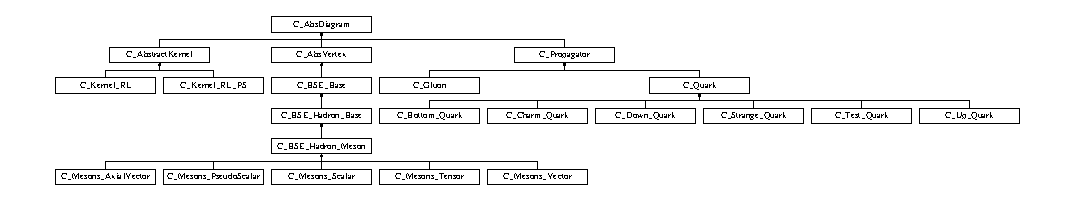
\includegraphics[height=2.248996cm]{class_c___abs_diagram}
\end{center}
\end{figure}
\subsection*{Public Member Functions}
\begin{DoxyCompactItemize}
\item 
\hypertarget{class_c___abs_diagram_a88baf4e9d29753417b7e65ef18f0b28f}{void {\bfseries Set\-Name\-I\-D} (string \-\_\-name, int \-\_\-\-I\-D)}\label{class_c___abs_diagram_a88baf4e9d29753417b7e65ef18f0b28f}

\item 
\hypertarget{class_c___abs_diagram_a5a52da1cfd635da06a6bfdd002e7f674}{void {\bfseries Get\-Name\-I\-D} ()}\label{class_c___abs_diagram_a5a52da1cfd635da06a6bfdd002e7f674}

\end{DoxyCompactItemize}
\subsection*{Protected Attributes}
\begin{DoxyCompactItemize}
\item 
\hypertarget{class_c___abs_diagram_a919d23735a009dc5a78e02e01e1eb40b}{string {\bfseries name}}\label{class_c___abs_diagram_a919d23735a009dc5a78e02e01e1eb40b}

\item 
\hypertarget{class_c___abs_diagram_a08de955405ee0344287b2eb5f6cb62b5}{int {\bfseries I\-D}}\label{class_c___abs_diagram_a08de955405ee0344287b2eb5f6cb62b5}

\item 
\hypertarget{class_c___abs_diagram_a958ffee1be22aa70a0e2eb9fa44f5784}{Dirac\-Gamma \hyperlink{class_c___abs_diagram_a958ffee1be22aa70a0e2eb9fa44f5784}{Z}}\label{class_c___abs_diagram_a958ffee1be22aa70a0e2eb9fa44f5784}

\begin{DoxyCompactList}\small\item\em Dirac gamma matrices $ \gamma_\mu $. \end{DoxyCompactList}\item 
\hypertarget{class_c___abs_diagram_a4eded4aff0f19920d9ec52e2f5c63abf}{Dirac\-Gamma {\bfseries Y}}\label{class_c___abs_diagram_a4eded4aff0f19920d9ec52e2f5c63abf}

\item 
\hypertarget{class_c___abs_diagram_a31794dd2c315f6bf18e2908d669ccc61}{Dirac\-Gamma5 \hyperlink{class_c___abs_diagram_a31794dd2c315f6bf18e2908d669ccc61}{\-\_\-\-Y5}}\label{class_c___abs_diagram_a31794dd2c315f6bf18e2908d669ccc61}

\begin{DoxyCompactList}\small\item\em Dirac gamma matrix $ \gamma_5 $. \end{DoxyCompactList}\item 
\hypertarget{class_c___abs_diagram_ac4646ab596ff13dd531f28f755d3dd4e}{Dirac\-Sigma \hyperlink{class_c___abs_diagram_ac4646ab596ff13dd531f28f755d3dd4e}{S\-I\-G}}\label{class_c___abs_diagram_ac4646ab596ff13dd531f28f755d3dd4e}

\begin{DoxyCompactList}\small\item\em Dirac sigma matrix $ \sigma_{\mu\nu} $. \end{DoxyCompactList}\item 
\hypertarget{class_c___abs_diagram_a4daaf1d6cbcb0aa0bc93417eb11b49a4}{Metric\-Tensor \hyperlink{class_c___abs_diagram_a4daaf1d6cbcb0aa0bc93417eb11b49a4}{g}}\label{class_c___abs_diagram_a4daaf1d6cbcb0aa0bc93417eb11b49a4}

\begin{DoxyCompactList}\small\item\em Euclidean metric tensor $ g_{\mu\nu} $. \end{DoxyCompactList}\item 
\hypertarget{class_c___abs_diagram_aff57681049aaff10af1fd2a0151209b8}{t\-\_\-cmplx\-Dirac \hyperlink{class_c___abs_diagram_aff57681049aaff10af1fd2a0151209b8}{I}}\label{class_c___abs_diagram_aff57681049aaff10af1fd2a0151209b8}

\begin{DoxyCompactList}\small\item\em Unit matrix (4,4) in Dirac space. \end{DoxyCompactList}\item 
\hypertarget{class_c___abs_diagram_a49ab5b499fd64c4a196349730d4beda3}{t\-\_\-cmplx\-Dirac {\bfseries Y5}}\label{class_c___abs_diagram_a49ab5b499fd64c4a196349730d4beda3}

\item 
\hypertarget{class_c___abs_diagram_a3e24081668fb3198fd043dd291fba4c5}{double {\bfseries pi}}\label{class_c___abs_diagram_a3e24081668fb3198fd043dd291fba4c5}

\item 
\hypertarget{class_c___abs_diagram_aa3cfb09af9c9e81fa1af3a78b5d667a7}{t\-\_\-cmplx \hyperlink{class_c___abs_diagram_aa3cfb09af9c9e81fa1af3a78b5d667a7}{ii}}\label{class_c___abs_diagram_aa3cfb09af9c9e81fa1af3a78b5d667a7}

\begin{DoxyCompactList}\small\item\em Imaginary unit. \end{DoxyCompactList}\end{DoxyCompactItemize}


The documentation for this class was generated from the following file\-:\begin{DoxyCompactItemize}
\item 
source/\-Abs/Abs\-Diagram.\-hpp\end{DoxyCompactItemize}

\input{class_c___abstract_builder}
\input{class_kernels_1_1_c___abstract_kernel}
\input{class_interpolation_1_1_c___bary_rat__interp}
\input{class_interpolation_1_1_c___base__interp}
\input{class_c___binder}
\input{class_propagators_1_1_c___bottom___quark}
\input{class_b_s_e_1_1_c___bound_state__parameters}
\input{class_b_s_e_1_1_c___b_s_e}
\input{class_b_s_e_1_1_c___b_s_e___factory}
\input{class_b_s_e_1_1_c___b_s_e___matrix}
\input{class_b_s_e_1_1_c___b_s_e___pseudo_scalar}
\input{class_b_s_e_1_1_c___b_s_e___scalar}
\input{class_b_s_e_1_1_c___b_s_e___two_body}
\input{class_b_s_e_1_1_c___b_s_e___vector}
\input{class_propagators_1_1_c___charm___quark}
\hypertarget{class_c___dedic_mem___abs}{\section{C\-\_\-\-Dedic\-Mem\-\_\-\-Abs Class Reference}
\label{class_c___dedic_mem___abs}\index{C\-\_\-\-Dedic\-Mem\-\_\-\-Abs@{C\-\_\-\-Dedic\-Mem\-\_\-\-Abs}}
}
Inheritance diagram for C\-\_\-\-Dedic\-Mem\-\_\-\-Abs\-:\begin{figure}[H]
\begin{center}
\leavevmode
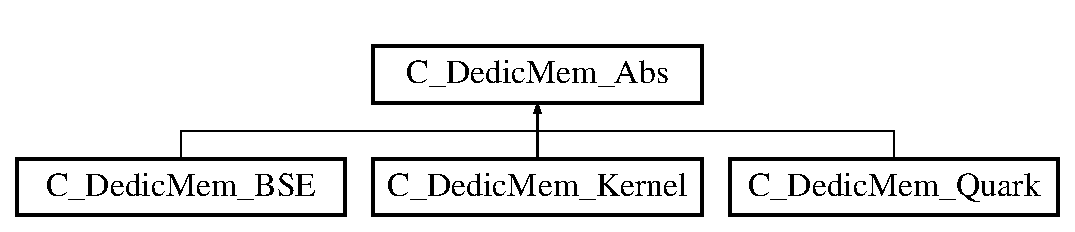
\includegraphics[height=2.000000cm]{class_c___dedic_mem___abs}
\end{center}
\end{figure}
\subsection*{Public Member Functions}
\begin{DoxyCompactItemize}
\item 
\hypertarget{class_c___dedic_mem___abs_a058cad18bf5cbc3e4d20272e41158f86}{virtual void {\bfseries info} ()=0}\label{class_c___dedic_mem___abs_a058cad18bf5cbc3e4d20272e41158f86}

\end{DoxyCompactItemize}


The documentation for this class was generated from the following file\-:\begin{DoxyCompactItemize}
\item 
source/\-Dedic\-Mem/Dedic\-Mem.\-hpp\end{DoxyCompactItemize}

\hypertarget{class_c___dedic_mem___b_s_e}{\section{C\-\_\-\-Dedic\-Mem\-\_\-\-B\-S\-E Class Reference}
\label{class_c___dedic_mem___b_s_e}\index{C\-\_\-\-Dedic\-Mem\-\_\-\-B\-S\-E@{C\-\_\-\-Dedic\-Mem\-\_\-\-B\-S\-E}}
}
Inheritance diagram for C\-\_\-\-Dedic\-Mem\-\_\-\-B\-S\-E\-:\begin{figure}[H]
\begin{center}
\leavevmode
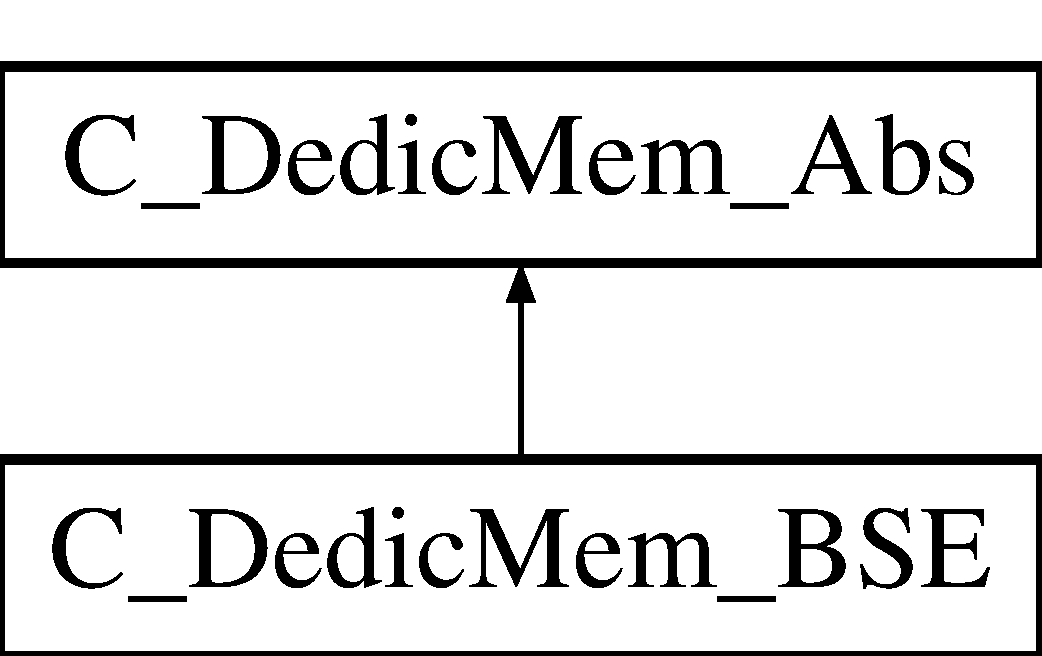
\includegraphics[height=2.000000cm]{class_c___dedic_mem___b_s_e}
\end{center}
\end{figure}
\subsection*{Public Member Functions}
\begin{DoxyCompactItemize}
\item 
\hypertarget{class_c___dedic_mem___b_s_e_ad6928f35d1bb6dc0a9e7896cb435de77}{void {\bfseries resize\-Amp\-Storage} (int amps, int points)}\label{class_c___dedic_mem___b_s_e_ad6928f35d1bb6dc0a9e7896cb435de77}

\item 
\hypertarget{class_c___dedic_mem___b_s_e_ae0fc9faee6bf0212366e272929d05299}{void {\bfseries set\-Amp\-Storage} (int amp, int point, t\-\_\-cmplx\-Dirac $\ast$Amp)}\label{class_c___dedic_mem___b_s_e_ae0fc9faee6bf0212366e272929d05299}

\item 
\hypertarget{class_c___dedic_mem___b_s_e_a1e45518a37fafeb43d866fdf8b60dbd6}{t\-\_\-cmplx\-Dirac {\bfseries get\-Amp\-Storage} (int amp, int point)}\label{class_c___dedic_mem___b_s_e_a1e45518a37fafeb43d866fdf8b60dbd6}

\item 
\hypertarget{class_c___dedic_mem___b_s_e_a832e259d5897e9b274d529979d92d08f}{void {\bfseries clear\-Amp\-Storage} ()}\label{class_c___dedic_mem___b_s_e_a832e259d5897e9b274d529979d92d08f}

\item 
\hypertarget{class_c___dedic_mem___b_s_e_a4e6c97cc94e185ccb93b4b83a6caa986}{void {\bfseries Resize\-E\-V\-Matrix} (int num\-\_\-rad, int num\-\_\-angle, int num\-\_\-amplitudes, int num\-\_\-chebs)}\label{class_c___dedic_mem___b_s_e_a4e6c97cc94e185ccb93b4b83a6caa986}

\item 
\hypertarget{class_c___dedic_mem___b_s_e_a77dd95cd06387357599deb84c8a1b5f3}{void {\bfseries resize\-B\-S\-E\-Contour} (int num\-\_\-amplitudes, int num\-\_\-points)}\label{class_c___dedic_mem___b_s_e_a77dd95cd06387357599deb84c8a1b5f3}

\item 
\hypertarget{class_c___dedic_mem___b_s_e_a1acb22de1a69296a075dc76a066c1cff}{void {\bfseries resize\-B\-S\-E\-Grid} (int num\-\_\-amplitudes, int num\-\_\-ex, int num\-\_\-in)}\label{class_c___dedic_mem___b_s_e_a1acb22de1a69296a075dc76a066c1cff}

\item 
\hypertarget{class_c___dedic_mem___b_s_e_a8eb9828cf1137c08d65e9c531f57dd87}{void {\bfseries clear\-Cauchy\-Grid} ()}\label{class_c___dedic_mem___b_s_e_a8eb9828cf1137c08d65e9c531f57dd87}

\item 
\hypertarget{class_c___dedic_mem___b_s_e_a7db75e75c587b9a25e937bb77ee399d7}{void {\bfseries info} ()}\label{class_c___dedic_mem___b_s_e_a7db75e75c587b9a25e937bb77ee399d7}

\end{DoxyCompactItemize}
\subsection*{Public Attributes}
\begin{DoxyCompactItemize}
\item 
\hypertarget{class_c___dedic_mem___b_s_e_a532449af372b4823ec11c1bac16a39f6}{std\-::vector$<$ std\-::vector\\*
$<$ t\-\_\-cmplx\-Dirac $>$ $>$ {\bfseries Amp\-Storage}}\label{class_c___dedic_mem___b_s_e_a532449af372b4823ec11c1bac16a39f6}

\item 
\hypertarget{class_c___dedic_mem___b_s_e_a5f0de44c8872d59b5db86058088e040e}{Eigen\-::\-Matrix\-Xcf {\bfseries E\-V\-Matrix}}\label{class_c___dedic_mem___b_s_e_a5f0de44c8872d59b5db86058088e040e}

\item 
\hypertarget{class_c___dedic_mem___b_s_e_adcbf7c4206df13acafeab297bc039f29}{t\-\_\-cmplx\-Array2\-D {\bfseries Cauchy\-Contour}}\label{class_c___dedic_mem___b_s_e_adcbf7c4206df13acafeab297bc039f29}

\item 
\hypertarget{class_c___dedic_mem___b_s_e_a0d11282e491e4762101a83d7e80e5733}{t\-\_\-cmplx\-Array3\-D {\bfseries Cauchy\-Grid}}\label{class_c___dedic_mem___b_s_e_a0d11282e491e4762101a83d7e80e5733}

\end{DoxyCompactItemize}


The documentation for this class was generated from the following files\-:\begin{DoxyCompactItemize}
\item 
source/\-Dedic\-Mem/Dedic\-Mem.\-hpp\item 
source/\-Dedic\-Mem/Dedic\-Mem.\-cpp\end{DoxyCompactItemize}

\hypertarget{class_c___dedic_mem___kernel}{\section{C\-\_\-\-Dedic\-Mem\-\_\-\-Kernel Class Reference}
\label{class_c___dedic_mem___kernel}\index{C\-\_\-\-Dedic\-Mem\-\_\-\-Kernel@{C\-\_\-\-Dedic\-Mem\-\_\-\-Kernel}}
}


{\ttfamily \#include $<$Dedic\-Mem.\-hpp$>$}

Inheritance diagram for C\-\_\-\-Dedic\-Mem\-\_\-\-Kernel\-:\begin{figure}[H]
\begin{center}
\leavevmode
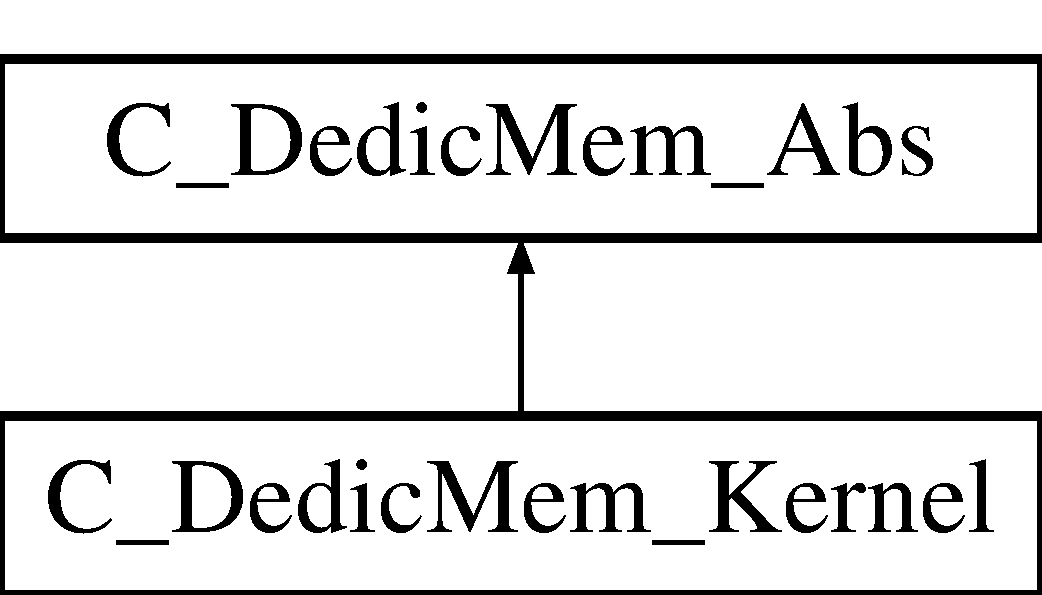
\includegraphics[height=2.000000cm]{class_c___dedic_mem___kernel}
\end{center}
\end{figure}
\subsection*{Public Member Functions}
\begin{DoxyCompactItemize}
\item 
void \hyperlink{class_c___dedic_mem___kernel_aa51b1668792ba7e0f843b2d03deb5819}{info} ()
\item 
void \hyperlink{class_c___dedic_mem___kernel_a53112d51dde01d8b4bd8f48ccce36a91}{Resize\-Kstorage} (int i)
\item 
void \hyperlink{class_c___dedic_mem___kernel_ac2013ecffb5dab674a568ef256f5a3f8}{Set\-Kmatrix\-At} (int i, \hyperlink{types_8h_ab0ebabce2061a9cbb83363a282add98f}{t\-\_\-cmplx\-Matrix2\-D} $\ast$\-\_\-\-K)
\item 
void \hyperlink{class_c___dedic_mem___kernel_ae8436015627826c00ef38c038ef829f8}{Erase\-Kstorage} ()
\item 
\hyperlink{types_8h_ab0ebabce2061a9cbb83363a282add98f}{t\-\_\-cmplx\-Matrix2\-D} $\ast$ \hyperlink{class_c___dedic_mem___kernel_aa95a927579efd2c095634e813c0db40f}{Get\-Kmatrix\-At} (int i)
\end{DoxyCompactItemize}
\subsection*{Public Attributes}
\begin{DoxyCompactItemize}
\item 
\hyperlink{types_8h_a71e866ee00a3173697327849014bce9b}{t\-\_\-cmplx\-Array4\-D} \hyperlink{class_c___dedic_mem___kernel_a1b2fcfb12ebf53baed1105d05c61f5fb}{Vertex\-Dressings}
\end{DoxyCompactItemize}


\subsection{Member Function Documentation}
\hypertarget{class_c___dedic_mem___kernel_ae8436015627826c00ef38c038ef829f8}{\index{C\-\_\-\-Dedic\-Mem\-\_\-\-Kernel@{C\-\_\-\-Dedic\-Mem\-\_\-\-Kernel}!Erase\-Kstorage@{Erase\-Kstorage}}
\index{Erase\-Kstorage@{Erase\-Kstorage}!C_DedicMem_Kernel@{C\-\_\-\-Dedic\-Mem\-\_\-\-Kernel}}
\subsubsection[{Erase\-Kstorage}]{\setlength{\rightskip}{0pt plus 5cm}void C\-\_\-\-Dedic\-Mem\-\_\-\-Kernel\-::\-Erase\-Kstorage (
\begin{DoxyParamCaption}
{}
\end{DoxyParamCaption}
)}}\label{class_c___dedic_mem___kernel_ae8436015627826c00ef38c038ef829f8}
\hypertarget{class_c___dedic_mem___kernel_aa95a927579efd2c095634e813c0db40f}{\index{C\-\_\-\-Dedic\-Mem\-\_\-\-Kernel@{C\-\_\-\-Dedic\-Mem\-\_\-\-Kernel}!Get\-Kmatrix\-At@{Get\-Kmatrix\-At}}
\index{Get\-Kmatrix\-At@{Get\-Kmatrix\-At}!C_DedicMem_Kernel@{C\-\_\-\-Dedic\-Mem\-\_\-\-Kernel}}
\subsubsection[{Get\-Kmatrix\-At}]{\setlength{\rightskip}{0pt plus 5cm}{\bf t\-\_\-cmplx\-Matrix2\-D} $\ast$ C\-\_\-\-Dedic\-Mem\-\_\-\-Kernel\-::\-Get\-Kmatrix\-At (
\begin{DoxyParamCaption}
\item[{int}]{i}
\end{DoxyParamCaption}
)}}\label{class_c___dedic_mem___kernel_aa95a927579efd2c095634e813c0db40f}
\hypertarget{class_c___dedic_mem___kernel_aa51b1668792ba7e0f843b2d03deb5819}{\index{C\-\_\-\-Dedic\-Mem\-\_\-\-Kernel@{C\-\_\-\-Dedic\-Mem\-\_\-\-Kernel}!info@{info}}
\index{info@{info}!C_DedicMem_Kernel@{C\-\_\-\-Dedic\-Mem\-\_\-\-Kernel}}
\subsubsection[{info}]{\setlength{\rightskip}{0pt plus 5cm}void C\-\_\-\-Dedic\-Mem\-\_\-\-Kernel\-::info (
\begin{DoxyParamCaption}
{}
\end{DoxyParamCaption}
)\hspace{0.3cm}{\ttfamily [virtual]}}}\label{class_c___dedic_mem___kernel_aa51b1668792ba7e0f843b2d03deb5819}


Implements \hyperlink{class_c___dedic_mem___abs_a058cad18bf5cbc3e4d20272e41158f86}{C\-\_\-\-Dedic\-Mem\-\_\-\-Abs}.

\hypertarget{class_c___dedic_mem___kernel_a53112d51dde01d8b4bd8f48ccce36a91}{\index{C\-\_\-\-Dedic\-Mem\-\_\-\-Kernel@{C\-\_\-\-Dedic\-Mem\-\_\-\-Kernel}!Resize\-Kstorage@{Resize\-Kstorage}}
\index{Resize\-Kstorage@{Resize\-Kstorage}!C_DedicMem_Kernel@{C\-\_\-\-Dedic\-Mem\-\_\-\-Kernel}}
\subsubsection[{Resize\-Kstorage}]{\setlength{\rightskip}{0pt plus 5cm}void C\-\_\-\-Dedic\-Mem\-\_\-\-Kernel\-::\-Resize\-Kstorage (
\begin{DoxyParamCaption}
\item[{int}]{i}
\end{DoxyParamCaption}
)}}\label{class_c___dedic_mem___kernel_a53112d51dde01d8b4bd8f48ccce36a91}
\hypertarget{class_c___dedic_mem___kernel_ac2013ecffb5dab674a568ef256f5a3f8}{\index{C\-\_\-\-Dedic\-Mem\-\_\-\-Kernel@{C\-\_\-\-Dedic\-Mem\-\_\-\-Kernel}!Set\-Kmatrix\-At@{Set\-Kmatrix\-At}}
\index{Set\-Kmatrix\-At@{Set\-Kmatrix\-At}!C_DedicMem_Kernel@{C\-\_\-\-Dedic\-Mem\-\_\-\-Kernel}}
\subsubsection[{Set\-Kmatrix\-At}]{\setlength{\rightskip}{0pt plus 5cm}void C\-\_\-\-Dedic\-Mem\-\_\-\-Kernel\-::\-Set\-Kmatrix\-At (
\begin{DoxyParamCaption}
\item[{int}]{i, }
\item[{{\bf t\-\_\-cmplx\-Matrix2\-D} $\ast$}]{\-\_\-\-K}
\end{DoxyParamCaption}
)}}\label{class_c___dedic_mem___kernel_ac2013ecffb5dab674a568ef256f5a3f8}


\subsection{Member Data Documentation}
\hypertarget{class_c___dedic_mem___kernel_a1b2fcfb12ebf53baed1105d05c61f5fb}{\index{C\-\_\-\-Dedic\-Mem\-\_\-\-Kernel@{C\-\_\-\-Dedic\-Mem\-\_\-\-Kernel}!Vertex\-Dressings@{Vertex\-Dressings}}
\index{Vertex\-Dressings@{Vertex\-Dressings}!C_DedicMem_Kernel@{C\-\_\-\-Dedic\-Mem\-\_\-\-Kernel}}
\subsubsection[{Vertex\-Dressings}]{\setlength{\rightskip}{0pt plus 5cm}{\bf t\-\_\-cmplx\-Array4\-D} C\-\_\-\-Dedic\-Mem\-\_\-\-Kernel\-::\-Vertex\-Dressings}}\label{class_c___dedic_mem___kernel_a1b2fcfb12ebf53baed1105d05c61f5fb}


The documentation for this class was generated from the following files\-:\begin{DoxyCompactItemize}
\item 
source/\-Dedic\-Mem/\hyperlink{_dedic_mem_8hpp}{Dedic\-Mem.\-hpp}\item 
source/\-Dedic\-Mem/\hyperlink{_dedic_mem_8cpp}{Dedic\-Mem.\-cpp}\end{DoxyCompactItemize}

\hypertarget{class_c___dedic_mem___quark}{\section{C\-\_\-\-Dedic\-Mem\-\_\-\-Quark Class Reference}
\label{class_c___dedic_mem___quark}\index{C\-\_\-\-Dedic\-Mem\-\_\-\-Quark@{C\-\_\-\-Dedic\-Mem\-\_\-\-Quark}}
}


{\ttfamily \#include $<$Dedic\-Mem.\-hpp$>$}

Inheritance diagram for C\-\_\-\-Dedic\-Mem\-\_\-\-Quark\-:\begin{figure}[H]
\begin{center}
\leavevmode
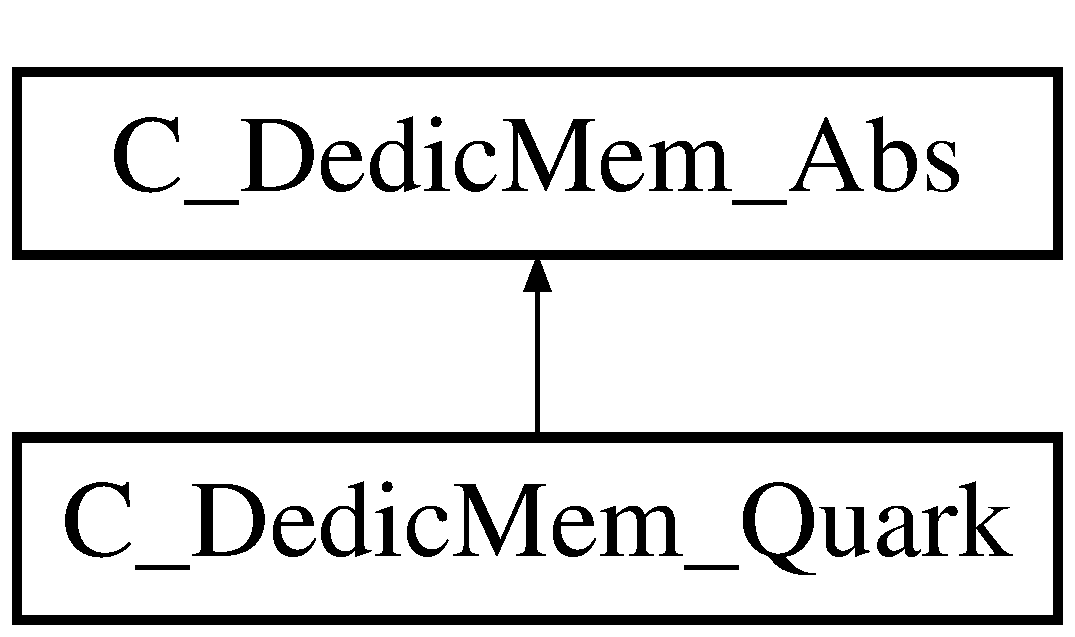
\includegraphics[height=2.000000cm]{class_c___dedic_mem___quark}
\end{center}
\end{figure}
\subsection*{Public Member Functions}
\begin{DoxyCompactItemize}
\item 
void \hyperlink{class_c___dedic_mem___quark_af9870170bb87b11db976c64fa2ff87bb}{resize\-Grid} (int amps\-\_\-num, int exter\-\_\-num, int inter\-\_\-num)
\item 
void \hyperlink{class_c___dedic_mem___quark_af25f857d41fa0b568af4a11218580729}{resize\-Contour} (int amps\-\_\-num, int cont\-\_\-num)
\item 
void \hyperlink{class_c___dedic_mem___quark_a868c98c7d5930a7fd0b4314d79092581}{Remove\-Grid} ()
\item 
void \hyperlink{class_c___dedic_mem___quark_aa2c1bd42ef41a11746d8ab96dcc70e75}{Remove\-Contour} ()
\item 
void \hyperlink{class_c___dedic_mem___quark_a7252d680bbd53e5c9a183fa49117d2e3}{info} ()
\end{DoxyCompactItemize}
\subsection*{Public Attributes}
\begin{DoxyCompactItemize}
\item 
\hyperlink{types_8h_a13088102853997a3c148dfe29c372f85}{t\-\_\-cmplx\-Array3\-D} \hyperlink{class_c___dedic_mem___quark_abb615a8d4eb2c5844634ac810197ad61}{S\-\_\-grid}
\item 
\hyperlink{types_8h_a4db8c78f1689c3a957b2866daaae58f2}{t\-\_\-cmplx\-Array2\-D} \hyperlink{class_c___dedic_mem___quark_a211eb01b6fb3e276987b2a99899d18b6}{S\-\_\-cont}
\end{DoxyCompactItemize}


\subsection{Member Function Documentation}
\hypertarget{class_c___dedic_mem___quark_a7252d680bbd53e5c9a183fa49117d2e3}{\index{C\-\_\-\-Dedic\-Mem\-\_\-\-Quark@{C\-\_\-\-Dedic\-Mem\-\_\-\-Quark}!info@{info}}
\index{info@{info}!C_DedicMem_Quark@{C\-\_\-\-Dedic\-Mem\-\_\-\-Quark}}
\subsubsection[{info}]{\setlength{\rightskip}{0pt plus 5cm}void C\-\_\-\-Dedic\-Mem\-\_\-\-Quark\-::info (
\begin{DoxyParamCaption}
{}
\end{DoxyParamCaption}
)\hspace{0.3cm}{\ttfamily [virtual]}}}\label{class_c___dedic_mem___quark_a7252d680bbd53e5c9a183fa49117d2e3}


Implements \hyperlink{class_c___dedic_mem___abs_a058cad18bf5cbc3e4d20272e41158f86}{C\-\_\-\-Dedic\-Mem\-\_\-\-Abs}.

\hypertarget{class_c___dedic_mem___quark_aa2c1bd42ef41a11746d8ab96dcc70e75}{\index{C\-\_\-\-Dedic\-Mem\-\_\-\-Quark@{C\-\_\-\-Dedic\-Mem\-\_\-\-Quark}!Remove\-Contour@{Remove\-Contour}}
\index{Remove\-Contour@{Remove\-Contour}!C_DedicMem_Quark@{C\-\_\-\-Dedic\-Mem\-\_\-\-Quark}}
\subsubsection[{Remove\-Contour}]{\setlength{\rightskip}{0pt plus 5cm}void C\-\_\-\-Dedic\-Mem\-\_\-\-Quark\-::\-Remove\-Contour (
\begin{DoxyParamCaption}
{}
\end{DoxyParamCaption}
)}}\label{class_c___dedic_mem___quark_aa2c1bd42ef41a11746d8ab96dcc70e75}
\hypertarget{class_c___dedic_mem___quark_a868c98c7d5930a7fd0b4314d79092581}{\index{C\-\_\-\-Dedic\-Mem\-\_\-\-Quark@{C\-\_\-\-Dedic\-Mem\-\_\-\-Quark}!Remove\-Grid@{Remove\-Grid}}
\index{Remove\-Grid@{Remove\-Grid}!C_DedicMem_Quark@{C\-\_\-\-Dedic\-Mem\-\_\-\-Quark}}
\subsubsection[{Remove\-Grid}]{\setlength{\rightskip}{0pt plus 5cm}void C\-\_\-\-Dedic\-Mem\-\_\-\-Quark\-::\-Remove\-Grid (
\begin{DoxyParamCaption}
{}
\end{DoxyParamCaption}
)}}\label{class_c___dedic_mem___quark_a868c98c7d5930a7fd0b4314d79092581}
\hypertarget{class_c___dedic_mem___quark_af25f857d41fa0b568af4a11218580729}{\index{C\-\_\-\-Dedic\-Mem\-\_\-\-Quark@{C\-\_\-\-Dedic\-Mem\-\_\-\-Quark}!resize\-Contour@{resize\-Contour}}
\index{resize\-Contour@{resize\-Contour}!C_DedicMem_Quark@{C\-\_\-\-Dedic\-Mem\-\_\-\-Quark}}
\subsubsection[{resize\-Contour}]{\setlength{\rightskip}{0pt plus 5cm}void C\-\_\-\-Dedic\-Mem\-\_\-\-Quark\-::resize\-Contour (
\begin{DoxyParamCaption}
\item[{int}]{amps\-\_\-num, }
\item[{int}]{cont\-\_\-num}
\end{DoxyParamCaption}
)}}\label{class_c___dedic_mem___quark_af25f857d41fa0b568af4a11218580729}
\hypertarget{class_c___dedic_mem___quark_af9870170bb87b11db976c64fa2ff87bb}{\index{C\-\_\-\-Dedic\-Mem\-\_\-\-Quark@{C\-\_\-\-Dedic\-Mem\-\_\-\-Quark}!resize\-Grid@{resize\-Grid}}
\index{resize\-Grid@{resize\-Grid}!C_DedicMem_Quark@{C\-\_\-\-Dedic\-Mem\-\_\-\-Quark}}
\subsubsection[{resize\-Grid}]{\setlength{\rightskip}{0pt plus 5cm}void C\-\_\-\-Dedic\-Mem\-\_\-\-Quark\-::resize\-Grid (
\begin{DoxyParamCaption}
\item[{int}]{amps\-\_\-num, }
\item[{int}]{exter\-\_\-num, }
\item[{int}]{inter\-\_\-num}
\end{DoxyParamCaption}
)}}\label{class_c___dedic_mem___quark_af9870170bb87b11db976c64fa2ff87bb}


\subsection{Member Data Documentation}
\hypertarget{class_c___dedic_mem___quark_a211eb01b6fb3e276987b2a99899d18b6}{\index{C\-\_\-\-Dedic\-Mem\-\_\-\-Quark@{C\-\_\-\-Dedic\-Mem\-\_\-\-Quark}!S\-\_\-cont@{S\-\_\-cont}}
\index{S\-\_\-cont@{S\-\_\-cont}!C_DedicMem_Quark@{C\-\_\-\-Dedic\-Mem\-\_\-\-Quark}}
\subsubsection[{S\-\_\-cont}]{\setlength{\rightskip}{0pt plus 5cm}{\bf t\-\_\-cmplx\-Array2\-D} C\-\_\-\-Dedic\-Mem\-\_\-\-Quark\-::\-S\-\_\-cont}}\label{class_c___dedic_mem___quark_a211eb01b6fb3e276987b2a99899d18b6}
\hypertarget{class_c___dedic_mem___quark_abb615a8d4eb2c5844634ac810197ad61}{\index{C\-\_\-\-Dedic\-Mem\-\_\-\-Quark@{C\-\_\-\-Dedic\-Mem\-\_\-\-Quark}!S\-\_\-grid@{S\-\_\-grid}}
\index{S\-\_\-grid@{S\-\_\-grid}!C_DedicMem_Quark@{C\-\_\-\-Dedic\-Mem\-\_\-\-Quark}}
\subsubsection[{S\-\_\-grid}]{\setlength{\rightskip}{0pt plus 5cm}{\bf t\-\_\-cmplx\-Array3\-D} C\-\_\-\-Dedic\-Mem\-\_\-\-Quark\-::\-S\-\_\-grid}}\label{class_c___dedic_mem___quark_abb615a8d4eb2c5844634ac810197ad61}


The documentation for this class was generated from the following files\-:\begin{DoxyCompactItemize}
\item 
source/\-Dedic\-Mem/\hyperlink{_dedic_mem_8hpp}{Dedic\-Mem.\-hpp}\item 
source/\-Dedic\-Mem/\hyperlink{_dedic_mem_8cpp}{Dedic\-Mem.\-cpp}\end{DoxyCompactItemize}

\input{class_propagators_1_1_c___down___quark}
\input{class_propagators_1_1_c___gluon}
\input{class_propagators_1_1_c___gluon___factory}
\input{class_c___gradiend___descent}
\input{class_integration_1_1_c___integration_nodes}
\input{class_integration_1_1_c___integrator___line}
\input{class_integration_1_1_c___integrator___path}
\input{class_kernels_1_1_c___kernel___factory}
\input{class_kernels_1_1_c___kernel___r_l}
\input{class_kernels_1_1_c___kernel___r_l___p_s}
\hypertarget{class_c___kinematics__1loop}{\section{C\-\_\-\-Kinematics\-\_\-1loop Class Reference}
\label{class_c___kinematics__1loop}\index{C\-\_\-\-Kinematics\-\_\-1loop@{C\-\_\-\-Kinematics\-\_\-1loop}}
}
\subsection*{Public Member Functions}
\begin{DoxyCompactItemize}
\item 
\hypertarget{class_c___kinematics__1loop_ac8ea5c0bc49a996a39f5d9bb9be77938}{void {\bfseries Set\-Vector\-\_\-\-P} (t\-\_\-cmplx P\-\_\-v)}\label{class_c___kinematics__1loop_ac8ea5c0bc49a996a39f5d9bb9be77938}

\item 
\hypertarget{class_c___kinematics__1loop_a19d01bd7b6d4823e432fe4b6e93bb5cb}{void {\bfseries Set\-Vector\-\_\-\-K} (t\-\_\-cmplx K\-\_\-v)}\label{class_c___kinematics__1loop_a19d01bd7b6d4823e432fe4b6e93bb5cb}

\item 
\hypertarget{class_c___kinematics__1loop_af2e051a57be7c9f8b4f82c9c8075f66f}{void {\bfseries Set\-Vectors\-\_\-p} (t\-\_\-cmplx z\-\_\-ex, t\-\_\-cmplx p\-\_\-ex)}\label{class_c___kinematics__1loop_af2e051a57be7c9f8b4f82c9c8075f66f}

\item 
\hypertarget{class_c___kinematics__1loop_a5f1fac5360637bd87b4cf4cf29577e41}{void {\bfseries Set\-Vectors\-\_\-k} (double \-\_\-zetta, t\-\_\-cmplx x, t\-\_\-cmplx y, t\-\_\-cmplx z)}\label{class_c___kinematics__1loop_a5f1fac5360637bd87b4cf4cf29577e41}

\item 
\hypertarget{class_c___kinematics__1loop_aa93f0b39da69100d1801a9d525b65fff}{void {\bfseries Set\-Vectors\-\_\-q} ()}\label{class_c___kinematics__1loop_aa93f0b39da69100d1801a9d525b65fff}

\item 
\hypertarget{class_c___kinematics__1loop_a9d78b3129c3eefedb197f1fd13c341e7}{void {\bfseries Set\-Vestors\-\_\-k\-\_\-for\-\_\-\-S} (double \-\_\-zetta, t\-\_\-cmplx\-Vector \-\_\-k)}\label{class_c___kinematics__1loop_a9d78b3129c3eefedb197f1fd13c341e7}

\item 
\hypertarget{class_c___kinematics__1loop_a9ea61128f7fc8f0c43ba3a7ca649059f}{t\-\_\-cmplx\-Dirac {\bfseries Trans\-In} (t\-\_\-cmplx\-Dirac \-\_\-\-T, t\-\_\-cmplx\-Vector \-\_\-\-P)}\label{class_c___kinematics__1loop_a9ea61128f7fc8f0c43ba3a7ca649059f}

\item 
\hypertarget{class_c___kinematics__1loop_a45b0eef2d7c9f649c233db2ce066dc4d}{t\-\_\-cmplx\-Tensor {\bfseries Trans\-In} (t\-\_\-cmplx\-Vector \-\_\-\-T, t\-\_\-cmplx\-Vector \-\_\-\-P)}\label{class_c___kinematics__1loop_a45b0eef2d7c9f649c233db2ce066dc4d}

\item 
\hypertarget{class_c___kinematics__1loop_aaa11f269ac21aecf200909d0396ab3cd}{void {\bfseries Shift\-Momenta} (double \-\_\-zetta)}\label{class_c___kinematics__1loop_aaa11f269ac21aecf200909d0396ab3cd}

\end{DoxyCompactItemize}
\subsection*{Public Attributes}
\begin{DoxyCompactItemize}
\item 
\hypertarget{class_c___kinematics__1loop_a441371d7421f15ba8c87a0574fa93a84}{t\-\_\-cmplx\-Vector {\bfseries k}}\label{class_c___kinematics__1loop_a441371d7421f15ba8c87a0574fa93a84}

\item 
\hypertarget{class_c___kinematics__1loop_a1e1e134607b2cba06419dd2369c95844}{t\-\_\-cmplx\-Vector {\bfseries k\-\_\-\-T}}\label{class_c___kinematics__1loop_a1e1e134607b2cba06419dd2369c95844}

\item 
\hypertarget{class_c___kinematics__1loop_adc3d5c1f175ea9acf4581c14082f61b7}{t\-\_\-cmplx\-Vector {\bfseries q}}\label{class_c___kinematics__1loop_adc3d5c1f175ea9acf4581c14082f61b7}

\item 
\hypertarget{class_c___kinematics__1loop_a0161d7d82d26adecb78c780d8f63a4b4}{t\-\_\-cmplx\-Vector {\bfseries q\-\_\-\-T}}\label{class_c___kinematics__1loop_a0161d7d82d26adecb78c780d8f63a4b4}

\item 
\hypertarget{class_c___kinematics__1loop_ac1aa1c0e58c7468f3f7f5e382f9b259f}{t\-\_\-cmplx\-Vector {\bfseries p}}\label{class_c___kinematics__1loop_ac1aa1c0e58c7468f3f7f5e382f9b259f}

\item 
\hypertarget{class_c___kinematics__1loop_ad3543bce80581d08fdd9898bc2780218}{t\-\_\-cmplx\-Vector {\bfseries p\-\_\-\-T}}\label{class_c___kinematics__1loop_ad3543bce80581d08fdd9898bc2780218}

\item 
\hypertarget{class_c___kinematics__1loop_af8a67f32848dd55cb7706903d51e5d83}{t\-\_\-cmplx\-Vector {\bfseries P}}\label{class_c___kinematics__1loop_af8a67f32848dd55cb7706903d51e5d83}

\item 
\hypertarget{class_c___kinematics__1loop_a361f9f849cabd9b7ee0d19f994a62b22}{t\-\_\-cmplx\-Vector {\bfseries k\-\_\-p}}\label{class_c___kinematics__1loop_a361f9f849cabd9b7ee0d19f994a62b22}

\item 
\hypertarget{class_c___kinematics__1loop_ae8d0733aae6200bc13039028e67db380}{t\-\_\-cmplx\-Vector {\bfseries k\-\_\-m}}\label{class_c___kinematics__1loop_ae8d0733aae6200bc13039028e67db380}

\item 
\hypertarget{class_c___kinematics__1loop_a02279e39bd4696f1d69390a7bd2588b5}{t\-\_\-cmplx\-Vector {\bfseries K}}\label{class_c___kinematics__1loop_a02279e39bd4696f1d69390a7bd2588b5}

\item 
\hypertarget{class_c___kinematics__1loop_a16c83ab6f2b880b6642d7bfde3f664ec}{t\-\_\-cmplx {\bfseries p\-\_\-\-P}}\label{class_c___kinematics__1loop_a16c83ab6f2b880b6642d7bfde3f664ec}

\item 
\hypertarget{class_c___kinematics__1loop_a7c8dbeaa212afb08d32d7aa2b5effc00}{t\-\_\-cmplx {\bfseries k\-\_\-\-P}}\label{class_c___kinematics__1loop_a7c8dbeaa212afb08d32d7aa2b5effc00}

\item 
\hypertarget{class_c___kinematics__1loop_a073860fdef9170dfd10d125811d245a3}{t\-\_\-cmplx {\bfseries q\-\_\-\-P}}\label{class_c___kinematics__1loop_a073860fdef9170dfd10d125811d245a3}

\item 
\hypertarget{class_c___kinematics__1loop_aeaa8b30330959af96ffee0dd8c545dc0}{t\-\_\-cmplx {\bfseries p2}}\label{class_c___kinematics__1loop_aeaa8b30330959af96ffee0dd8c545dc0}

\item 
\hypertarget{class_c___kinematics__1loop_aaf7a5dc2be4002c455d5bccbe4914c4a}{t\-\_\-cmplx {\bfseries k2}}\label{class_c___kinematics__1loop_aaf7a5dc2be4002c455d5bccbe4914c4a}

\item 
\hypertarget{class_c___kinematics__1loop_aac076faa327bf22e32ccf0123cb45636}{t\-\_\-cmplx {\bfseries q2}}\label{class_c___kinematics__1loop_aac076faa327bf22e32ccf0123cb45636}

\item 
\hypertarget{class_c___kinematics__1loop_a7dff81ad45ed5e4ea26244490912c52c}{t\-\_\-cmplx {\bfseries P2}}\label{class_c___kinematics__1loop_a7dff81ad45ed5e4ea26244490912c52c}

\item 
\hypertarget{class_c___kinematics__1loop_a384d988f7c660f8cb04a2eb3377084a2}{t\-\_\-cmplx {\bfseries p2\-\_\-\-T}}\label{class_c___kinematics__1loop_a384d988f7c660f8cb04a2eb3377084a2}

\item 
\hypertarget{class_c___kinematics__1loop_ae2ed8d22f5cc5340e4f59c708194169f}{t\-\_\-cmplx {\bfseries k2\-\_\-\-T}}\label{class_c___kinematics__1loop_ae2ed8d22f5cc5340e4f59c708194169f}

\item 
\hypertarget{class_c___kinematics__1loop_a5380c55913e80399964c32a5fe456dd7}{t\-\_\-cmplx {\bfseries q2\-\_\-\-T}}\label{class_c___kinematics__1loop_a5380c55913e80399964c32a5fe456dd7}

\item 
\hypertarget{class_c___kinematics__1loop_a33b6f88ce54ff6dfd7342d75974b91e1}{t\-\_\-cmplx {\bfseries N2\-\_\-\-Factor}}\label{class_c___kinematics__1loop_a33b6f88ce54ff6dfd7342d75974b91e1}

\end{DoxyCompactItemize}


The documentation for this class was generated from the following file\-:\begin{DoxyCompactItemize}
\item 
source/\-Abs/Kinematics.\-hpp\end{DoxyCompactItemize}

\hypertarget{class_geometry_1_1_c___line}{\section{Geometry\-:\-:C\-\_\-\-Line Class Reference}
\label{class_geometry_1_1_c___line}\index{Geometry\-::\-C\-\_\-\-Line@{Geometry\-::\-C\-\_\-\-Line}}
}
Inheritance diagram for Geometry\-:\-:C\-\_\-\-Line\-:\begin{figure}[H]
\begin{center}
\leavevmode
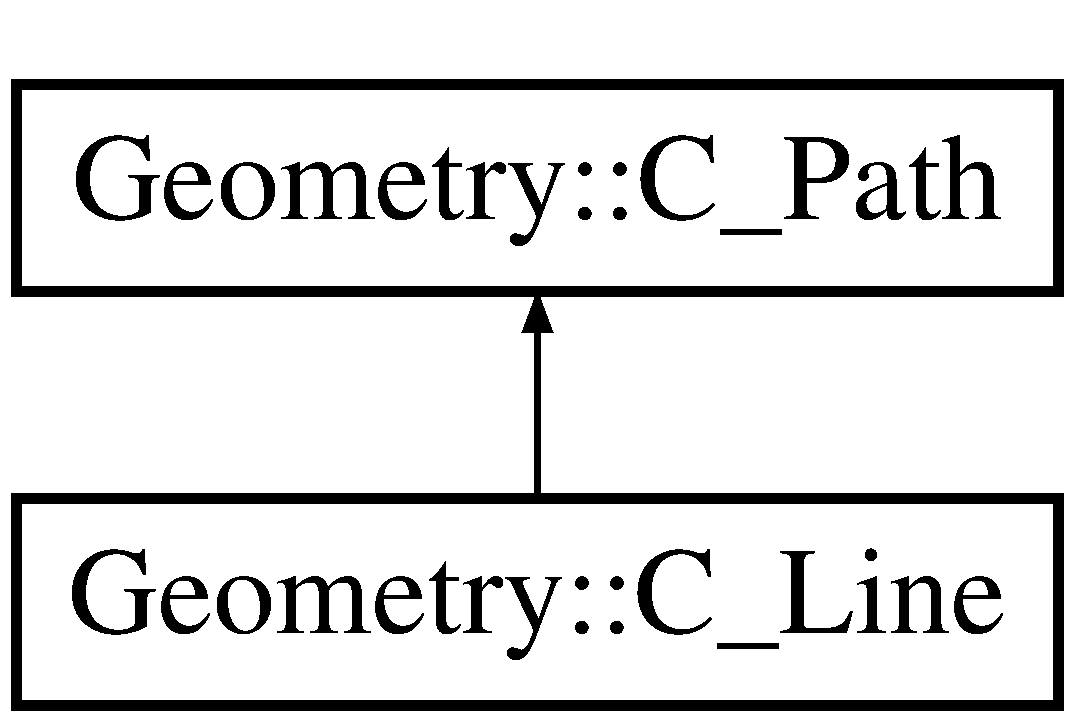
\includegraphics[height=2.000000cm]{class_geometry_1_1_c___line}
\end{center}
\end{figure}
\subsection*{Public Member Functions}
\begin{DoxyCompactItemize}
\item 
\hypertarget{class_geometry_1_1_c___line_a15acedc22ff33f4b92e3aa10d15081ed}{{\bfseries C\-\_\-\-Line} (t\-\_\-cmplx \-\_\-\-\_\-k\-\_\-coeff, t\-\_\-cmplx \-\_\-\-\_\-b\-\_\-coeff)}\label{class_geometry_1_1_c___line_a15acedc22ff33f4b92e3aa10d15081ed}

\item 
\hypertarget{class_geometry_1_1_c___line_a16c50bebf737fc6a12f9605be5c38944}{t\-\_\-cmplx {\bfseries get\-Path\-At} (t\-\_\-cmplx t\-\_\-paramtr)}\label{class_geometry_1_1_c___line_a16c50bebf737fc6a12f9605be5c38944}

\item 
\hypertarget{class_geometry_1_1_c___line_a5d2a8ca944731f6b8d239b9aa52cbfdf}{t\-\_\-cmplx {\bfseries get\-Derivative\-Path\-At} (t\-\_\-cmplx t\-\_\-paramtr)}\label{class_geometry_1_1_c___line_a5d2a8ca944731f6b8d239b9aa52cbfdf}

\end{DoxyCompactItemize}


The documentation for this class was generated from the following files\-:\begin{DoxyCompactItemize}
\item 
source/\-Num\-Libs/\-Geometry/Line.\-hpp\item 
source/\-Num\-Libs/\-Geometry/Line.\-cpp\end{DoxyCompactItemize}

\input{class_interpolation_1_1_c___linear}
\hypertarget{class_c___memory_factory___b_s_e}{\section{C\-\_\-\-Memory\-Factory\-\_\-\-B\-S\-E Class Reference}
\label{class_c___memory_factory___b_s_e}\index{C\-\_\-\-Memory\-Factory\-\_\-\-B\-S\-E@{C\-\_\-\-Memory\-Factory\-\_\-\-B\-S\-E}}
}


{\ttfamily \#include $<$Memory\-Factories.\-hpp$>$}

\subsection*{Public Member Functions}
\begin{DoxyCompactItemize}
\item 
\hyperlink{class_c___dedic_mem___abs}{C\-\_\-\-Dedic\-Mem\-\_\-\-Abs} $\ast$ \hyperlink{class_c___memory_factory___b_s_e_a75af4c2fa19fd6ccf7f046c323e005c2}{Create\-Memory} ()
\end{DoxyCompactItemize}


\subsection{Member Function Documentation}
\hypertarget{class_c___memory_factory___b_s_e_a75af4c2fa19fd6ccf7f046c323e005c2}{\index{C\-\_\-\-Memory\-Factory\-\_\-\-B\-S\-E@{C\-\_\-\-Memory\-Factory\-\_\-\-B\-S\-E}!Create\-Memory@{Create\-Memory}}
\index{Create\-Memory@{Create\-Memory}!C_MemoryFactory_BSE@{C\-\_\-\-Memory\-Factory\-\_\-\-B\-S\-E}}
\subsubsection[{Create\-Memory}]{\setlength{\rightskip}{0pt plus 5cm}{\bf C\-\_\-\-Dedic\-Mem\-\_\-\-Abs}$\ast$ C\-\_\-\-Memory\-Factory\-\_\-\-B\-S\-E\-::\-Create\-Memory (
\begin{DoxyParamCaption}
{}
\end{DoxyParamCaption}
)\hspace{0.3cm}{\ttfamily [inline]}}}\label{class_c___memory_factory___b_s_e_a75af4c2fa19fd6ccf7f046c323e005c2}


The documentation for this class was generated from the following file\-:\begin{DoxyCompactItemize}
\item 
source/\-Dedic\-Mem/\hyperlink{_memory_factories_8hpp}{Memory\-Factories.\-hpp}\end{DoxyCompactItemize}

\hypertarget{class_c___memory_factory___kernel}{\section{C\-\_\-\-Memory\-Factory\-\_\-\-Kernel Class Reference}
\label{class_c___memory_factory___kernel}\index{C\-\_\-\-Memory\-Factory\-\_\-\-Kernel@{C\-\_\-\-Memory\-Factory\-\_\-\-Kernel}}
}
Inheritance diagram for C\-\_\-\-Memory\-Factory\-\_\-\-Kernel\-:\begin{figure}[H]
\begin{center}
\leavevmode
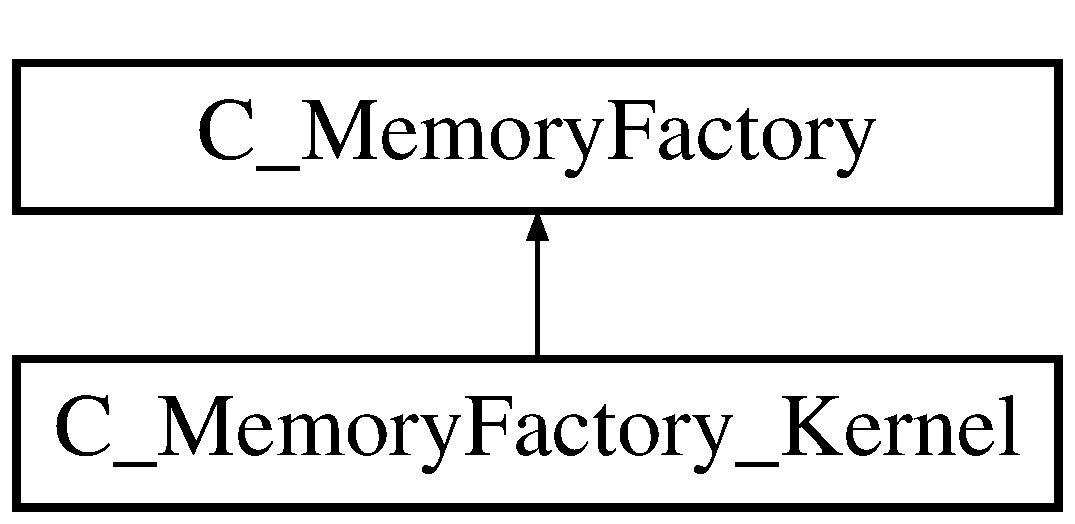
\includegraphics[height=2.000000cm]{class_c___memory_factory___kernel}
\end{center}
\end{figure}
\subsection*{Public Member Functions}
\begin{DoxyCompactItemize}
\item 
\hypertarget{class_c___memory_factory___kernel_ac8741e6e30ed5dad51579507cf7b4007}{\hyperlink{class_c___dedic_mem___abs}{C\-\_\-\-Dedic\-Mem\-\_\-\-Abs} $\ast$ {\bfseries Create\-Memory} ()}\label{class_c___memory_factory___kernel_ac8741e6e30ed5dad51579507cf7b4007}

\end{DoxyCompactItemize}


The documentation for this class was generated from the following file\-:\begin{DoxyCompactItemize}
\item 
source/\-Dedic\-Mem/Memory\-Factories.\-hpp\end{DoxyCompactItemize}

\hypertarget{class_c___memory_factory___quark}{\section{C\-\_\-\-Memory\-Factory\-\_\-\-Quark Class Reference}
\label{class_c___memory_factory___quark}\index{C\-\_\-\-Memory\-Factory\-\_\-\-Quark@{C\-\_\-\-Memory\-Factory\-\_\-\-Quark}}
}
Inheritance diagram for C\-\_\-\-Memory\-Factory\-\_\-\-Quark\-:\begin{figure}[H]
\begin{center}
\leavevmode
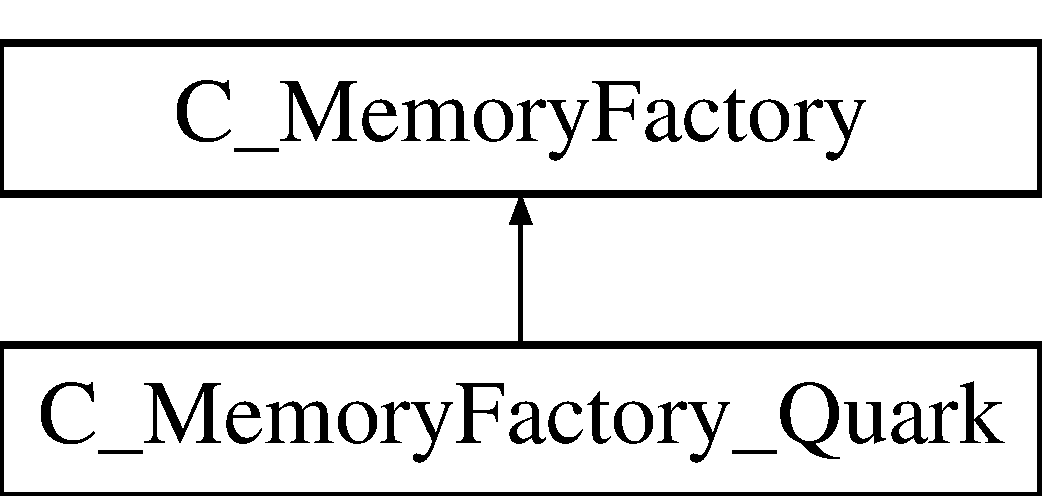
\includegraphics[height=2.000000cm]{class_c___memory_factory___quark}
\end{center}
\end{figure}
\subsection*{Public Member Functions}
\begin{DoxyCompactItemize}
\item 
\hypertarget{class_c___memory_factory___quark_acdd015023349f6658c14cd5f74d1806d}{\hyperlink{class_c___dedic_mem___abs}{C\-\_\-\-Dedic\-Mem\-\_\-\-Abs} $\ast$ {\bfseries Create\-Memory} ()}\label{class_c___memory_factory___quark_acdd015023349f6658c14cd5f74d1806d}

\end{DoxyCompactItemize}


The documentation for this class was generated from the following file\-:\begin{DoxyCompactItemize}
\item 
source/\-Dedic\-Mem/Memory\-Factories.\-hpp\end{DoxyCompactItemize}

\input{class_c___meson_builder}
\input{class_integration_1_1_c___one_loop_integrator}
\hypertarget{class_geometry_1_1_c___parabola}{\section{Geometry\-:\-:C\-\_\-\-Parabola Class Reference}
\label{class_geometry_1_1_c___parabola}\index{Geometry\-::\-C\-\_\-\-Parabola@{Geometry\-::\-C\-\_\-\-Parabola}}
}
Inheritance diagram for Geometry\-:\-:C\-\_\-\-Parabola\-:\begin{figure}[H]
\begin{center}
\leavevmode
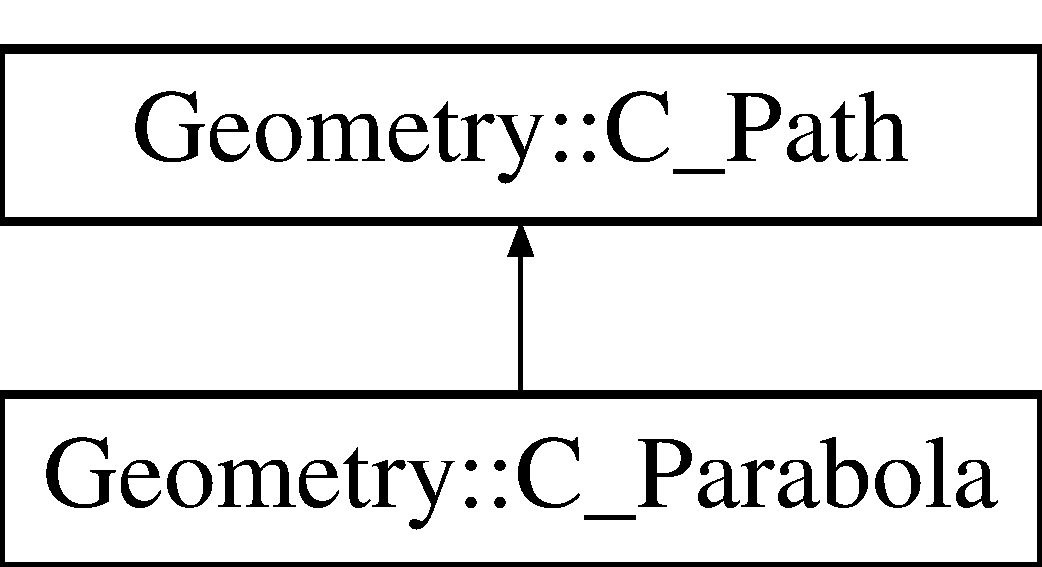
\includegraphics[height=2.000000cm]{class_geometry_1_1_c___parabola}
\end{center}
\end{figure}
\subsection*{Public Member Functions}
\begin{DoxyCompactItemize}
\item 
\hypertarget{class_geometry_1_1_c___parabola_af2dbf3b230334f8c68a116dbe6d21490}{{\bfseries C\-\_\-\-Parabola} (t\-\_\-cmplx \-\_\-\-\_\-\-Parabola\-Apex)}\label{class_geometry_1_1_c___parabola_af2dbf3b230334f8c68a116dbe6d21490}

\item 
\hypertarget{class_geometry_1_1_c___parabola_a387364d860d1fdd83294af454635acb0}{t\-\_\-cmplx {\bfseries get\-Path\-At} (t\-\_\-cmplx t\-\_\-paramtr)}\label{class_geometry_1_1_c___parabola_a387364d860d1fdd83294af454635acb0}

\item 
\hypertarget{class_geometry_1_1_c___parabola_a783b277435ef183353620f94471e3d7d}{t\-\_\-cmplx {\bfseries get\-Derivative\-Path\-At} (t\-\_\-cmplx t\-\_\-paramtr)}\label{class_geometry_1_1_c___parabola_a783b277435ef183353620f94471e3d7d}

\end{DoxyCompactItemize}


The documentation for this class was generated from the following files\-:\begin{DoxyCompactItemize}
\item 
source/\-Num\-Libs/\-Geometry/Parabola.\-hpp\item 
source/\-Num\-Libs/\-Geometry/Parabola.\-cpp\end{DoxyCompactItemize}

\hypertarget{class_geometry_1_1_c___parabola_contour}{\section{Geometry\-:\-:C\-\_\-\-Parabola\-Contour Class Reference}
\label{class_geometry_1_1_c___parabola_contour}\index{Geometry\-::\-C\-\_\-\-Parabola\-Contour@{Geometry\-::\-C\-\_\-\-Parabola\-Contour}}
}
\subsection*{Public Member Functions}
\begin{DoxyCompactItemize}
\item 
\hypertarget{class_geometry_1_1_c___parabola_contour_aa0c00c9315f7d61dd1731074e0846dba}{{\bfseries C\-\_\-\-Parabola\-Contour} (t\-\_\-cmplx \-\_\-\-\_\-\-Parabola\-Apex, t\-\_\-cmplx \-\_\-\-\_\-k\-\_\-coeff, t\-\_\-cmplx \-\_\-\-\_\-b\-\_\-coeff)}\label{class_geometry_1_1_c___parabola_contour_aa0c00c9315f7d61dd1731074e0846dba}

\item 
\hypertarget{class_geometry_1_1_c___parabola_contour_a578b2b2d45be66ef6effe03cbf047a7a}{void {\bfseries set\-Parabola\-Contour} (const t\-\_\-d\-Array1\-D \&p\-\_\-parabola, const t\-\_\-d\-Array1\-D \&w\-\_\-parabola, const t\-\_\-d\-Array1\-D \&p\-\_\-line, const t\-\_\-d\-Array1\-D \&w\-\_\-line)}\label{class_geometry_1_1_c___parabola_contour_a578b2b2d45be66ef6effe03cbf047a7a}

\item 
\hypertarget{class_geometry_1_1_c___parabola_contour_a32867584ce7dfc8234a3446fa803c23f}{t\-\_\-cmplx\-Array2\-D {\bfseries get\-Parabola\-Contour} ()}\label{class_geometry_1_1_c___parabola_contour_a32867584ce7dfc8234a3446fa803c23f}

\end{DoxyCompactItemize}


The documentation for this class was generated from the following files\-:\begin{DoxyCompactItemize}
\item 
source/\-Num\-Libs/\-Geometry/Parabola\-Contour.\-hpp\item 
source/\-Num\-Libs/\-Geometry/Parabola\-Contour.\-cpp\end{DoxyCompactItemize}

\hypertarget{class_geometry_1_1_c___path}{\section{Geometry\-:\-:C\-\_\-\-Path Class Reference}
\label{class_geometry_1_1_c___path}\index{Geometry\-::\-C\-\_\-\-Path@{Geometry\-::\-C\-\_\-\-Path}}
}
Inheritance diagram for Geometry\-:\-:C\-\_\-\-Path\-:\begin{figure}[H]
\begin{center}
\leavevmode
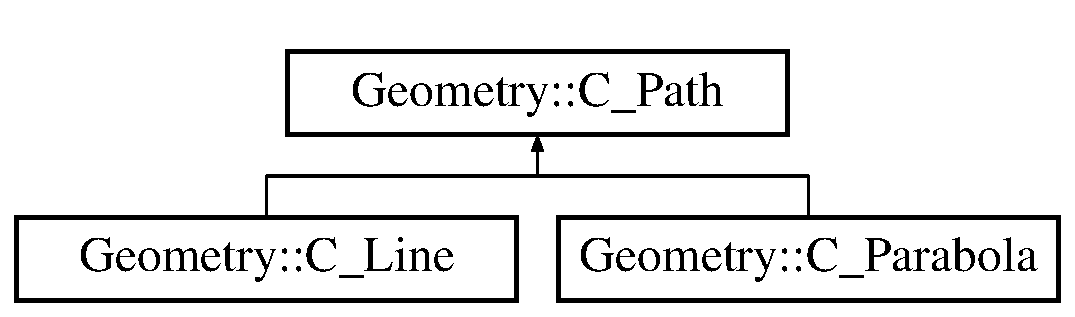
\includegraphics[height=2.000000cm]{class_geometry_1_1_c___path}
\end{center}
\end{figure}
\subsection*{Public Member Functions}
\begin{DoxyCompactItemize}
\item 
\hypertarget{class_geometry_1_1_c___path_a3e09ce3608385b63ebbe9ffad0f0599b}{t\-\_\-cmplx\-Array1\-D {\bfseries get\-Path\-On\-Vector} (t\-\_\-cmplx\-Array1\-D Sample\-Points)}\label{class_geometry_1_1_c___path_a3e09ce3608385b63ebbe9ffad0f0599b}

\item 
\hypertarget{class_geometry_1_1_c___path_a133c937a36b957116043fddfe3fedf46}{virtual t\-\_\-cmplx {\bfseries get\-Path\-At} (t\-\_\-cmplx t\-\_\-paramtr)}\label{class_geometry_1_1_c___path_a133c937a36b957116043fddfe3fedf46}

\item 
\hypertarget{class_geometry_1_1_c___path_a62acb86d6a96d7f0a3185fb498ec449d}{virtual t\-\_\-cmplx {\bfseries get\-Derivative\-Path\-At} (t\-\_\-cmplx t\-\_\-paramtr)}\label{class_geometry_1_1_c___path_a62acb86d6a96d7f0a3185fb498ec449d}

\end{DoxyCompactItemize}


The documentation for this class was generated from the following files\-:\begin{DoxyCompactItemize}
\item 
source/\-Num\-Libs/\-Geometry/Path.\-hpp\item 
source/\-Num\-Libs/\-Geometry/Path.\-cpp\end{DoxyCompactItemize}

\input{class_propagators_1_1_c___propagator}
\input{class_propagators_1_1_c___quark}
\input{class_propagators_1_1_c___quark___factory}
\input{class_propagators_1_1_c___quark__parameters}
\input{class_c___spectra}
\input{class_propagators_1_1_c___strange___quark}
\input{class_propagators_1_1_c___test___quark}
\input{class_kernels_1_1_c___two_quark_kernel}
\input{class_propagators_1_1_c___up___quark}
\chapter{File Documentation}
\input{mainpage_8dox}
\input{_abs_diagram_8hpp}
\input{_kinematics_8hpp}
\input{_bound_state__parameters_8cpp}
\input{_bound_state__parameters_8h}
\input{_b_s_e_8h}
\input{_b_s_e___factory_8h}
\input{_b_s_e___matrix_8cpp}
\input{_b_s_e___matrix_8h}
\input{_b_s_e___pseudo_scalar_8cpp}
\input{_b_s_e___pseudo_scalar_8h}
\input{_b_s_e___scalar_8cpp}
\input{_b_s_e___scalar_8h}
\input{_b_s_e___two_body_8cpp}
\input{_b_s_e___two_body_8h}
\input{_b_s_e___vector_8cpp}
\input{_b_s_e___vector_8h}
\input{_dedic_mem_8cpp}
\input{_dedic_mem_8hpp}
\input{_memory_factories_8cpp}
\input{_memory_factories_8hpp}
\input{_gluon_8cpp}
\input{_gluon_8hpp}
\input{_propagator_8cpp}
\input{_propagator_8hpp}
\input{_propagator_factory_8hpp}
\input{_quark_8cpp}
\input{_quark_8hpp}
\input{_quark__parameters_8cpp}
\input{_quark__parameters_8hpp}
\input{_quark_types_8hpp}
\input{_d_s_epp_8hpp}
\input{_example_8cpp}
\input{_abstract_kernel_8hpp}
\input{_kernel_factory_8hpp}
\input{_rainbow_ladder_kernel_8cpp}
\input{_rainbow_ladder_kernel_8hpp}
\input{_r_land_pseudo_scalar_8cpp}
\input{_r_land_pseudo_scalar_8hpp}
\input{_two_quark_kernel_8hpp}
\input{_barycentric_interpolation_8h}
\input{_chebychev_polinoms_8h}
\input{_extra__functions_8h}
\input{_line_8cpp}
\input{_line_8hpp}
\input{_parabola_8cpp}
\input{_parabola_8hpp}
\input{_parabola_contour_8cpp}
\input{_parabola_contour_8hpp}
\input{_path_8cpp}
\input{_path_8hpp}
\input{_gradiend_descent_8h}
\input{_integration_nodes_8hpp}
\input{_integrator_8hpp}
\input{_integrator___path_8hpp}
\input{_linear_interpolation_8h}
\input{_one_loop_integrator_8hpp}
\input{_abstract_builder_8cpp}
\input{_abstract_builder_8h}
\input{_binder_8cpp}
\input{_binder_8h}
\input{_meson_builder_8cpp}
\input{_meson_builder_8h}
\input{_spectra_8cpp}
\input{_spectra_8h}
\input{types_8h}
%--- End generated contents ---

% Index
\newpage
\phantomsection
\addcontentsline{toc}{chapter}{Index}
\printindex

\end{document}
